\documentclass[../../main.tex]{subfiles}

\begin{document}

Und das Rechnen mit negativen Zahlen besser zu verstehen, haben wir uns im Kapitel über 
\hyperlink{chap:ganzezahlen}{\emph{ganze Zahlen}} die Addition und Subtraktion von Zahlen mithilfe von Zahlengeraden
veranschaulicht. Die beiden folgenden Bilder zeigen zum Beispiel, wie wir zu zwei verschiedenen Zahlen $+3$ addieren
können: $-2+3=1$ und $0+3=3$.

\begin{multicols}{2}
\centering

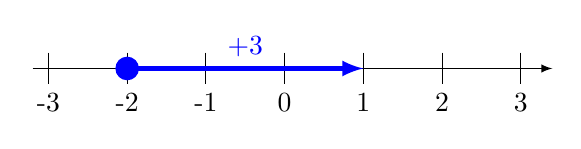
\begin{tikzpicture}
    \draw[-latex] (-3.2,0) -- (3.4,0);
    \foreach \x in {-3,...,3}{
        \draw (\x,0.2) -- (\x,-0.2) node[below] {\x};
    }
    \draw[blue,ultra thick,-latex] (-2,0) -- node[above] {$+3$} (1,0);
    \fill[blue] (-2,0) circle[radius=1.5mm];
\end{tikzpicture}

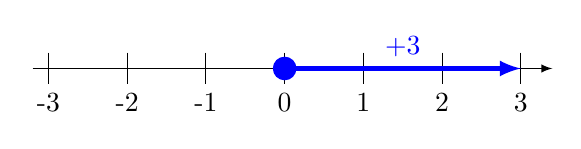
\begin{tikzpicture}
    \draw[-latex] (-3.2,0) -- (3.4,0);
    \foreach \x in {-3,...,3}{
        \draw (\x,0.2) -- (\x,-0.2) node[below] {\x};
    }
    \draw[blue,ultra thick,-latex] (0,0) -- node[above] {$+3$} (3,0);
    \fill[blue] (0,0) circle[radius=1.5mm];
\end{tikzpicture}

\end{multicols}

Anschaulich verschieben wir eine Zahl immer um 3 nach rechts, wenn wir $+3$ zu ihr addieren. In beiden Bildern gibt
der blaue Pfeil also die Richtung an, in die wir eine Zahl verschieben müssen, um $+3$ zu addieren. Das funktioniert,
egal wo wir mit dem Pfeil starten. Wenn wir beschreiben wollen, wie der Pfeil aussieht, benötigen wir damit nur seine
Länge und seine Richtung, nicht aber seinen genauen Ort.

Das Ziel in diesem Kapitel wird es sein, Pfeile wie im obigen Bild sinnvoll beschreiben zu können, mit ihnen zu rechnen 
und sie zu verwenden, um zwei- und dreidimensionale Objekte zu beschreiben. Weil die Pfeile nur Richtungen darstellen,
müssen wir nur zwei Dinge über den Pfeil wissen:
\begin{itemize}
    \item Wie lang ist der Pfeil?
    \item In welche Richtung zeigt der Pfeil?
\end{itemize}
In unserem Fall reicht eine einzige Zahl, nämlich die 3, um uns diese Information zu geben: 3 ist eine positive Zahl,
also zeigt der Pfeil nach rechts (bei einer negativen Zahl würde der Pfeil nach links zeigen), und zwar genau drei 
Schritte. Entsprechend würde $-2$ den Pfeil beschreiben, der zwei Schritte nach links zeigt.

\parpic[r]{
    \begin{tikzpicture}
        \begin{axis}[defgrid, domain=0:4, y=1cm, x=1cm, ymin=0, ymax=3, xmin=0, xmax=4, xtick={1,...,4}, ytick={1,...,4}]
            \draw[-latex, ultra thick, blue!60] (1,1) -- node[above] {$v$} (3,2);
        \end{axis}
    \end{tikzpicture}
}
\picskip{8}
Schauen wir uns nun an, wie sich unsere Situation ändert, wenn unsere Pfeile nicht nur nach links oder rechts, sondern
in eine beliebige Richtung zeigen dürfen. Dafür vervollständigen wir die Zahlengerade, die wir oben gesehen haben, zu
einem Koordinatensystem. Wie können wir nun den Pfeil $v$ beschreiben, der rechts im Koordinatensystem zu sehen ist?

Auf der Zahlengerade mussten wir ausschließlich angeben, wie weit der Pfeil nach rechts bzw. links zeigt. Da der Pfeil
jetzt zusätzlich nach oben oder unten verlaufen kann, benötigen wir noch zusätzlich die Information, wie viele Schritte
der Pfeil nach oben zeigt (dabei bedeuten negative Zahlen wieder, dass der Pfeil nach unten zeigt). Ins unserem Fall
führt der blaue Pfeil zwei Schritte nach rechts und einen nach oben. Wir schreiben für einen solchen Pfeil dann 
$v=\vectwo{2}{1}$ und meinen damit, dass $v$ ein Pfeil ist, der zwei Schritte nach rechts (erster Eintrag) und einen 
Schritt nach oben (zweiter Eintrag) führt. Wie schon erwähnt, gibt dies \emph{ausschließlich die Richtung, aber nicht 
den Startpunkt} des Pfeils an. Die folgenden Pfeile werden ebenfalls durch $v_1=v_2=v_3=\vectwo{2}{1}$ beschrieben -- 
wir sehen sie alle als gleich an, weil der Startpunkt uns nicht interessiert.
\begin{multicols}{3}
    \begin{tikzpicture}
        \begin{axis}[defgrid, domain=0:4, y=1cm, x=1cm, ymin=0, ymax=3, xmin=0, xmax=4, xtick={1,...,4}, ytick={1,...,4}]
            \draw[-latex, ultra thick, blue!60] (0,0) -- node[above] {$v_1$} (2,1);
        \end{axis}
    \end{tikzpicture}
    \begin{tikzpicture}
        \begin{axis}[defgrid, domain=0:4, y=1cm, x=1cm, ymin=0, ymax=3, xmin=0, xmax=4, xtick={1,...,4}, ytick={1,...,4}]
            \draw[-latex, ultra thick, blue!60] (2,2) -- node[above] {$v_2$} (4,3);
        \end{axis}
    \end{tikzpicture}
    \begin{tikzpicture}
        \begin{axis}[defgrid, domain=0:4, y=1cm, x=1cm, ymin=0, ymax=3, xmin=0, xmax=4, xtick={1,...,4}, ytick={1,...,4}]
            \draw[-latex, ultra thick, blue!60] (1,0) -- node[above] {$v_3$} (3,1);
        \end{axis}
    \end{tikzpicture}
\end{multicols}
Pfeile, die wir auf diese Art beschreiben, nennen wir \textbf{Vektoren}. Wir versuchen nun, den Vektor $v=\vectwo{2}{1}$ 
so zu modifizieren, dass seine Richtung gleich bleibt, aber die Länge größer oder kleiner wird. Unten siehst du drei
weitere Vektoren, die in die gleiche Richtung wie $v$ zeigen, aber jeweils länger oder kürzer sind. Der Vektor $a$ ist
zum Beispiel doppelt so lang wie $v$. Das heißt, dass er jeweils doppelt so viele Schritte nach rechts und oben führt wie $v$.
Um die Einträge des Vektors $a$ zu berechnen, können wir also alle Einträge von $v$ mit $2$ 
multiplizieren und erhalten
\[a=\vectwo{2\cdot 2}{2\cdot 1}=\vectwo{4}{2}.\]
Weil die Schreibweise in der Mitte etwas sperrig ist, schreiben wir die Zahl $2$, mit der wir alle Einträge
von $v$ multipliziert haben, nach vorn:
\[a=2\cdot\vectwo{2}{1}=\vectwo{4}{2}\]

\begin{multicols}{3}
    \begin{tikzpicture}
        \begin{axis}[defgrid, domain=0:4, y=1cm, x=1cm, ymin=0, ymax=3, xmin=0, xmax=4, xtick={1,...,4}, ytick={1,...,4}]
            \draw[-latex, ultra thick, green!70!black] (0,0) -- node[above] {$a$} (4,2);
        \end{axis}
    \end{tikzpicture}

    \begin{tikzpicture}
        \begin{axis}[defgrid, domain=0:4, y=1cm, x=1cm, ymin=0, ymax=3, xmin=0, xmax=4, xtick={1,...,4}, ytick={1,...,4}]
            \draw[-latex, ultra thick, red] (0,0) -- node[above] {$b$} (1,0.5);
        \end{axis}
    \end{tikzpicture}

    \begin{tikzpicture}
        \begin{axis}[defgrid, domain=-4:0, y=1cm, x=1cm, ymin=-3, ymax=0, xmin=-4, xmax=0, xtick={-4,...,-1}, ytick={-4,...,-1}]
            \draw[-latex, ultra thick, orange] (0,0) -- node[below] {$c$} (-2,-1);
        \end{axis}
    \end{tikzpicture}
\end{multicols}
Entsprechend erhalten wir auch die anderen Vektoren: $b$ ist halb so lang wie $v$, 
also $b=\frac{1}{2}\cdot\vectwo{2}{1}=\vectwo{\frac{1}{2}\cdot 2}{\frac{1}{2}\cdot 1}=\vectwo{1}{\frac{1}{2}}$. Der Vektor $c$ führt zwei Schritte nach links (dies
beschreiben wir mit dem Eintrag $-2$) und einen nach unten (also Eintrag $-1$). $c$ ist somit genau der Vektor, den wir
erhalten, wenn wir alle Einträge von $v$ mit $-1$ multiplizieren, also $c=-1\cdot\vectwo{2}{1}=\vectwo{-1\cdot 2}{-1\cdot 1}=\vectwo{-2}{-1}$. Er
sieht genau wie der Vektor $v$ aus -- mit dem Unterschied, dass wir Start- und Endpunkt vertauscht haben. Den Vorgang, 
einen Vektor mit einer Zahl $\lambda\in\R$ multiplizieren, also
\[\lambda\cdot\vectwo{v_1}{v_2}=\vectwo{\lambda\cdot v_1}{\lambda\cdot v_2},\]
nennen wir \textbf{Skalarmultiplikation} (im 
Umgang mit Vektoren nennt man einfache Zahlen, die selbst keine Vektoren sind, \textbf{Skalare}, hier ist also $\lambda$ ein \emph{Skalar}).
Bei der Skalarmultiplikation ändert sich lediglich die Länge des Vektors, aber nie seine Richtung. Genauer haben wir 
Folgendes beobachtet:
\begin{itemize}
    \item Ist $\abs{\lambda}>1$, so ist der Vektor $\lambda\cdot v$ länger als $v$.
    \item Ist $\abs{\lambda}<1$, so ist der Vektor $\lambda\cdot v$ kürzer als $v$.
    \item Ist $\lambda<0$, so dreht die Skalarmultiplikation mit $\lambda$ den Vektor $v$ um.
\end{itemize}
\parpic[r]{
    \begin{tikzpicture}
        \begin{axis}[defgrid, domain=0:4, y=1cm, x=1cm, ymin=0, ymax=3, xmin=0, xmax=4, xtick={1,...,4}, ytick={1,...,4}]
            \draw[-latex, ultra thick, orange] (0,1) -- node[above] {$a$} (3,2);
            \draw[-latex, ultra thick, green!70!black] (3,2) -- node[right] {$b$} (4,0);
            \draw[-latex, ultra thick, gray] (0,1) -- node[above] {$a+b$} (4,0);
        \end{axis}
    \end{tikzpicture}
}
Als nächstes untersuchen wir, was passiert, wenn wir zwei Vektoren wie rechts abgebildet hintereinander hängen, also so,
dass der zweite Vektor bei der Pfeilspitze des ersten Vektors beginnt. Folgen wir erst der Richtung des Vektors $a=\vectwo{3}{1}$ und
dann der Richtung des Vektors $b=\vectwo{1}{-2}$, dann legen wir nach rechts erst drei Schritte, dann einen zurück,
insgesamt also $3+1=4$. Auf die gleiche Weise machen wir erst einen Schritt nach oben, dann zwei nach unten, also
insgesamt einen Schritt nach unten. Damit lässt sich unsere Gesamtbewegung durch den Vektor 
\[a+b=\vectwo{3}{1}+\vectwo{1}{-2}=\vectwo{3+1}{1+(-2)}=\vectwo{4}{-1}\]
beschreiben. Wenn wir zwei Vektoren hintereinander hängen, bekommen wir insgesamt also eine Richtung, die genau der
Summe der beiden Vektoren entspricht.

Schließlich können wir zwei Vektoren auch voneinander subtrahieren. Dafür subtrahieren wir die einzelnen Einträge von 
einander, etwa
\[\vectwo{3}{1}-\vectwo{1}{-2}=\vectwo{3-1}{1-(-2)}=\vectwo{2}{3}.\]
Geometrisch drehen wir den zweiten Vektor dabei einfach einmal um, bevor wir ihn an den ersten hängen.

\parpic[r]{
    \begin{tikzpicture}
        \begin{axis}[defgrid, domain=0:4, y=1cm, x=1cm, ymin=0, ymax=3, xmin=0, xmax=5, xtick={1,...,5}, ytick={1,...,4}]
            \draw[-latex, ultra thick, blue!60] (0,1) -- node[above] {$v$} (3,3);
            \draw[-latex, ultra thick, green!70!black, dashed] (0,1) -- node[below] {$3$ Schritte} (3,1);
            \draw[-latex, ultra thick, gray, dashed] (3,1) -- node[right] {$2$ Schritte} (3,3);
        \end{axis}
    \end{tikzpicture}
}
\picskip{8}
Weil Vektoren nicht nur in eine bestimmte Richtung zeigen, sondern auch immer eine bestimmte Länge haben, ist unser 
letztes Ziel in diesem Abschnitt, herauszufinden, wie wir diese Länge berechnen können. Rechts siehst du den Vektor 
$v=\vectwo{3}{2}$, der 3 Schritte nach rechts und 2 Schritte nach oben zeigt. Zusammen mit den beiden gestrichelt
eingezeichneten Linien bildet $v$ ein rechtwinkliges Dreieck. Um die Länge von $v$ zu bestimmen, können wir jetzt
den Satz des Pythagoras verwenden:
\[3^2+2^2=\abs{v}^2\]
Da wir den Wert $\abs{v}$ anstelle des Wertes $\abs{v}^2$ berechnen wollen, müssen wir noch die Wurzel ziehen und erhalten
\[\abs{v}=\sqrt{3^2+2^2}=\sqrt{13}.\]
Die Formel, mit der wir die Länge eines Vektors $v=\vectwo{v_1}{v_2}$ berechnen können, lautet also
\[\abs{v}=\sqrt{v_1^2+v_2^2}.\]
\if 0
\begin{advanced}{$\R$-Vektorräume}
    Im Kapitel über Mengenlehre hast du das kartesische Produkt kennengelernt, mit dem sich aus gegebenen Mengen neue
    konstruieren lassen. Mit dem kartesischen Produkt können wir auch genauer beschreiben, aus welcher Menge unsere
    bisher verwendeten Vektoren stammen, nämlich aus
    \[\R^2:=\R\times\R=\{(x,y)\mid x,y\in\R\}.\]
    Wenn wir $\vectwo{x}{y}$ anstelle von $(x,y)$ schreiben, erhalten wir genau die Vektoren, die wir gerade eingeführt 
    haben. Wir haben bereits erklärt, wie sich die Elemente von $\R^2$ addieren und mit Elementen aus $\R$ multiplizieren
    lassen. Die Skalarmultiplikation und Vektoraddition erfüllen die folgenden Rechenregeln:

    \begin{multicols}{2}
        \begin{enumerate}
        \item $u+(v+w)=(u+v)+w$ für alle $u,v,w\in\R^2$
        \item $u+v=v+u$ für alle $u,v\in\R^2$
        \item Es existiert $0\in\R^2$, sodass für alle $v\in\R^2$ gilt: $0+v=v$
        \item Zu jedem $v\in\R^2$ existiert ein $v'\in\R^2$ mit $v+v'=0$
        \item $1\cdot v=v$ für alle $v\in\R^2$
        \item $\alpha\cdot (u+v)=\alpha\cdot u+\alpha\cdot v$ für alle $\alpha\in\R, u,v\in\R^2$
        \item $(\alpha+\beta)\cdot v=\alpha\cdot v+\beta\cdot v$ für alle $\alpha,\beta\in\R, v\in\R^2$
        \item $(\alpha\cdot\beta)\cdot v=\alpha\cdot (\beta\cdot v)$ für alle $\alpha,\beta\in\R,v\in\R^2$
        \end{enumerate}
    \end{multicols}
    Damit die Rechenregeln funktionieren, wählen wir $v'=-v$ und $0=\vectwo{0}{0}$. Der Vektor $-v$ heißt dann \textbf{inverses
    Element} von $v$ und der Vektor $\vectwo{0}{0}$ wird als \textbf{neutrales Element} bezeichnet.
    Jede Menge $V$, für die eine Vektoraddition und eine Skalarmultiplikation mit Elementen aus $\R$ mit diesen Eigenschaften
    existieren, heißt $\R$-Vektorraum (die Vektoren werden dann nicht aus der Menge $\R^2$, sondern aus der Menge $V$ 
    gewählt). Damit lässt sich das Konzept von Vektoren auf beliebig viele Einträge 
    verallgemeinern und
    \[\R^n:=\underbrace{\R\times\dots\times\R}_{n-\text{mal}}=\{(x_1,\dots,x_n)\mid x_1,\dots,x_n\in\R\}\]
    wird nach dem gleichen Prinzip wie $\R^2$ zu einem $\R$-Vektorraum. In den weiterführenden Aufgaben zu diesem 
    Abschnitt wirst du weitere Beispiele für $\R$-Vektorräume kennenlernen, die etwas anders funktionieren.
\end{advanced}
\fi
\begin{nutshell}{Was sind Vektoren?}
    \parpic[r]{
        \begin{tikzpicture}
            \begin{axis}[defgrid, domain=0:4, y=1cm, x=1cm, ymin=0, ymax=3, xmin=0, xmax=4, xtick={1,...,4}, ytick={1,...,4}]
                \draw[-latex, ultra thick, blue!60] (1,1) -- node[below] {$v=\vectwo{3}{2}$} (4,3);
            \end{axis}
        \end{tikzpicture}
    }
    \picskip{9}
    \textbf{Vektoren} werden verwendet, um Richtungen zu beschreiben. Wir können uns Vektoren als Pfeile in einem 
    Koordinatensystem vorstellen. Einen Vektor $v$ können wir beispielsweise folgendermaßen notieren:
    \[v=\vectwo{3}{2}\]
    Die obere Zahl gibt dabei an, wie viele Schritte der Vektor nach rechts führt und die untere Zahl gibt an, wie viele
    Schritte der Vektor nach oben führt. Während es bei Vektoren wichtig ist, wie lang sie sind, ist es egal, wo sich
    ihr Startpunkt befindet. Mit Vektoren können wir wie folgt rechnen:

    \vspace*{3mm}
    \begin{minipage}{5cm}
        \tikz{
            \begin{axis}[defgrid, domain=0:4, y=1cm, x=1cm, ymin=0, ymax=3, xmin=0, xmax=4, xtick={1,...,4}, ytick={1,...,4}]
                \draw[-latex, ultra thick, orange!30] (0,1) -- (4,3);
                \draw[-latex, ultra thick, orange!50] (0,1) -- (3.5,2.75);
                \draw[-latex, ultra thick, orange!70] (0,1) -- (3,2.5);
                \draw[-latex, ultra thick, orange] (0,1) -- node[above] {$u$} (2,2);
                \node at (3,2.9) {$\lambda\cdot u$};
                \draw[-latex, ultra thick, green!70!black] (2,2) -- node[right] {$v$} (4,0);
                \draw[-latex, ultra thick, gray] (0,1) -- node[above] {$u+v$} (4,0);
            \end{axis}
        }
        \end{minipage}
    \begin{itemize}
        \item Wir können Vektoren länger bzw. kürzer machen, ohne ihre Richtung zu verändern, indem wir sie mit einer Zahl $\lambda\in\R$ (in
        Abgrenzung zu Vektoren auch \textbf{Skalar} genannt) multiplizieren:
        \[\lambda\cdot \vectwo{v_1}{v_2}=\vectwo{\lambda\cdot v_1}{\lambda \cdot v_2}\]
        Ist $\lambda$ dabei negativ, drehen wir den Vektor bei der Multiplikation außerdem um.
        \item Wir können zwei Vektoren addieren, indem wir ihre Einträge addieren:
        \[\vectwo{u_1}{u_2}+\vectwo{v_1}{v_2}=\vectwo{u_1+v_1}{u_2+v_2}\]
        Dies gibt die Richtung an, die wir erhalten, wenn wir beide Vektoren hintereinander hängen.
        \item Der Vektor $v=\vectwo{v_1}{v_2}$ hat die Länge
        \[\abs{v}=\sqrt{v_1^2+v_2^2}.\]
    \end{itemize}
\end{nutshell}

\end{document}